\subsection*{Log ud}
I forlængelse af log ind funktionen, er det også en log ud funktion. Denne funktion tillader brugeren at logge sig ud af systemet, således at brugeren ikke forbliver logget ind, og tillader yderligere andre brugere at logge ind fra samme app.
Aktiviteterne for log ind funktion fremgår af \autoref{fig:logind}.

\begin{figure} [H]
\centering
\textbf{Aktivitetsdiagram: Log ud}\par\medskip
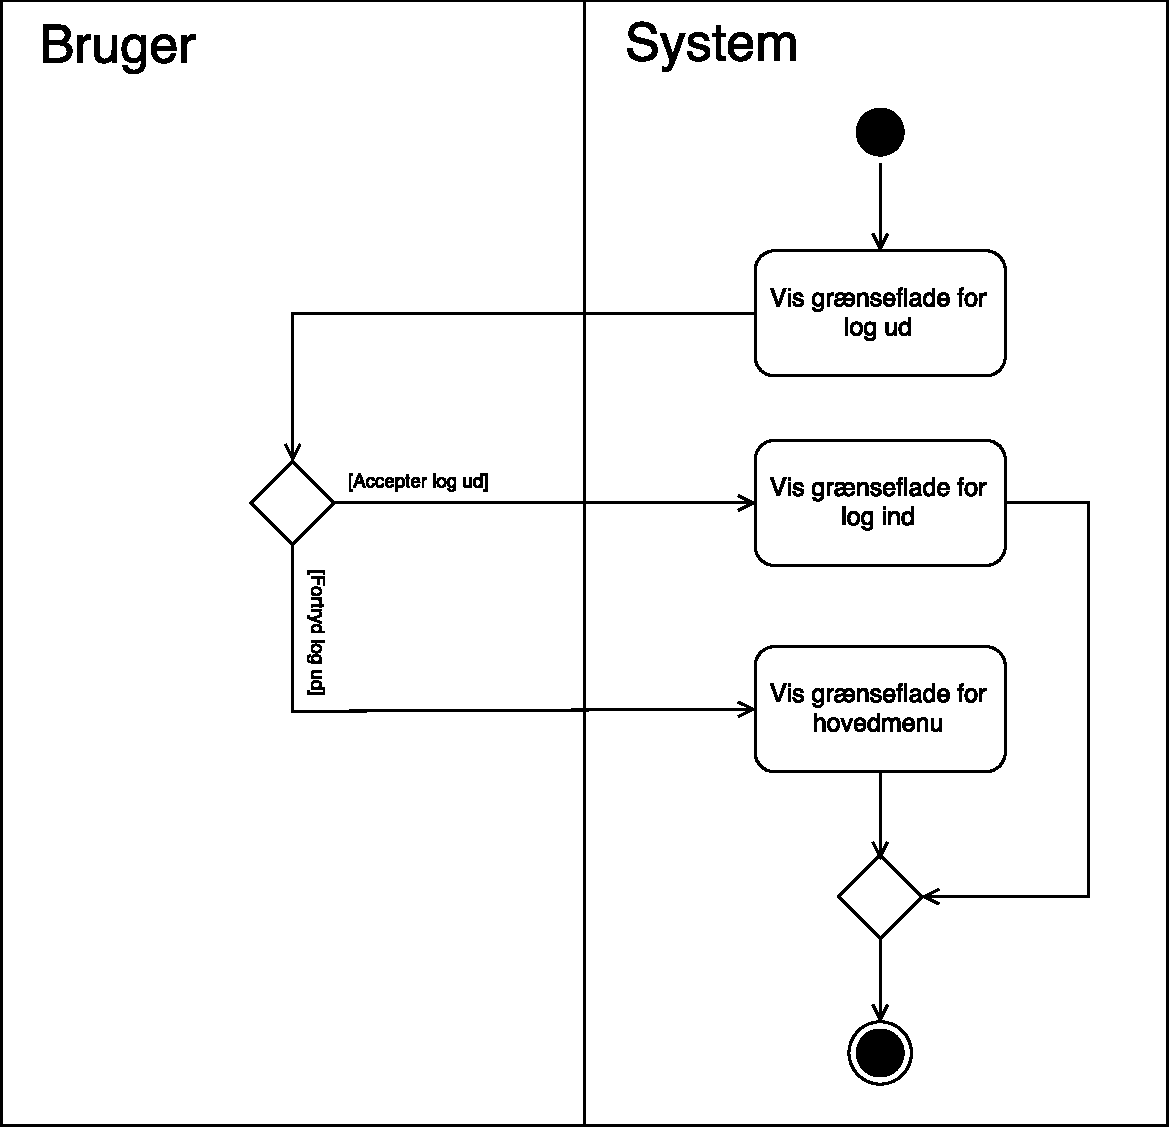
\includegraphics[width=0.9\textwidth]{figures/aktivitetsdiagram/Logud}
\caption{Aktivitetsdiagram over log ud, hvor aktiviteter forekommer hos brugen, systemet eller databasen.}
\label{fig:logud}
\end{figure}

Brugeren har fra hovedmenuen, muligheden for at logge ud af systemet. Vælger brugen dette, vil grænsefladen for log ud vises. 
Brugeren skal efterfølgende bekræfte at de ønsker at logge ud, før at systemet systemt gennemføre handlingen og vis grænsefladen for log ind. Brugeren kan dog også vælge at fortryde log ud handlingen, i tilfælde af at bruger ved fejl valgte log ud, hvor systemet vil returnere til hovedmenuen.  